\section{Results}
\label{sec:results}

\subsection{Mechanism Gate: SSD Approximation Strengthens with $N$ (RQ1)}

\begin{table}[h]
\centering
\caption{Normalized SSD Frobenius error at each sequence length.}
\label{tab:mechanism_gate}
\begin{tabular}{lrrrr}
\toprule
$N$ & $n$ & Mean Error/$N$ & Std/$N$ & 90th pct/$N$ \\
\midrule
512   & 1,600 & 0.0392 & 0.0071 & 0.0478 \\
1,024 & 160   & 0.0331 & 0.0057 & 0.0383 \\
2,048 & 160   & 0.0235 & 0.0043 & 0.0273 \\
\bottomrule
\end{tabular}
\end{table}

Log-log slope $\beta = \mathbf{-0.368}$ (threshold $\leq 0.5$ \checkmark).
90th pct at $N=2048 = \mathbf{0.027}$ (threshold $\leq 0.3$ \checkmark).
\textbf{Both gate criteria pass with large margin.}

Normalized error decreases by $\sim$23\% per doubling of $N$. Across all 32 LLaMA-3-8B layers,
no layer is an outlier. The error distribution shifts downward as $N$ increases
(Figure~\ref{fig:loglog}, Figure~\ref{fig:violin}).

\textbf{Interpretation:} SSD approximation quality is not the bottleneck. Any retrieval
degradation observed in H-E1 must be attributed to the bounded-state state update
$h_t = A \cdot h_{t-1} + B \cdot x_t$, which exponentially forgets early token positions
independently of how well SSD weights are aligned.

\textbf{Surprising finding:} The pre-registered threshold allowed sub-linear \emph{growth}
($\beta \leq 0.5$); the actual slope is negative ($\beta = -0.368$). We attribute this to
increasing attention sparsity at longer $N$: LLaMA-3-8B attention concentrates on fewer
positions at longer range (head specialization, diluted mass), creating a lower-rank
approximation target that fixed-rank SSD captures more efficiently.

\begin{figure}[h]
\centering
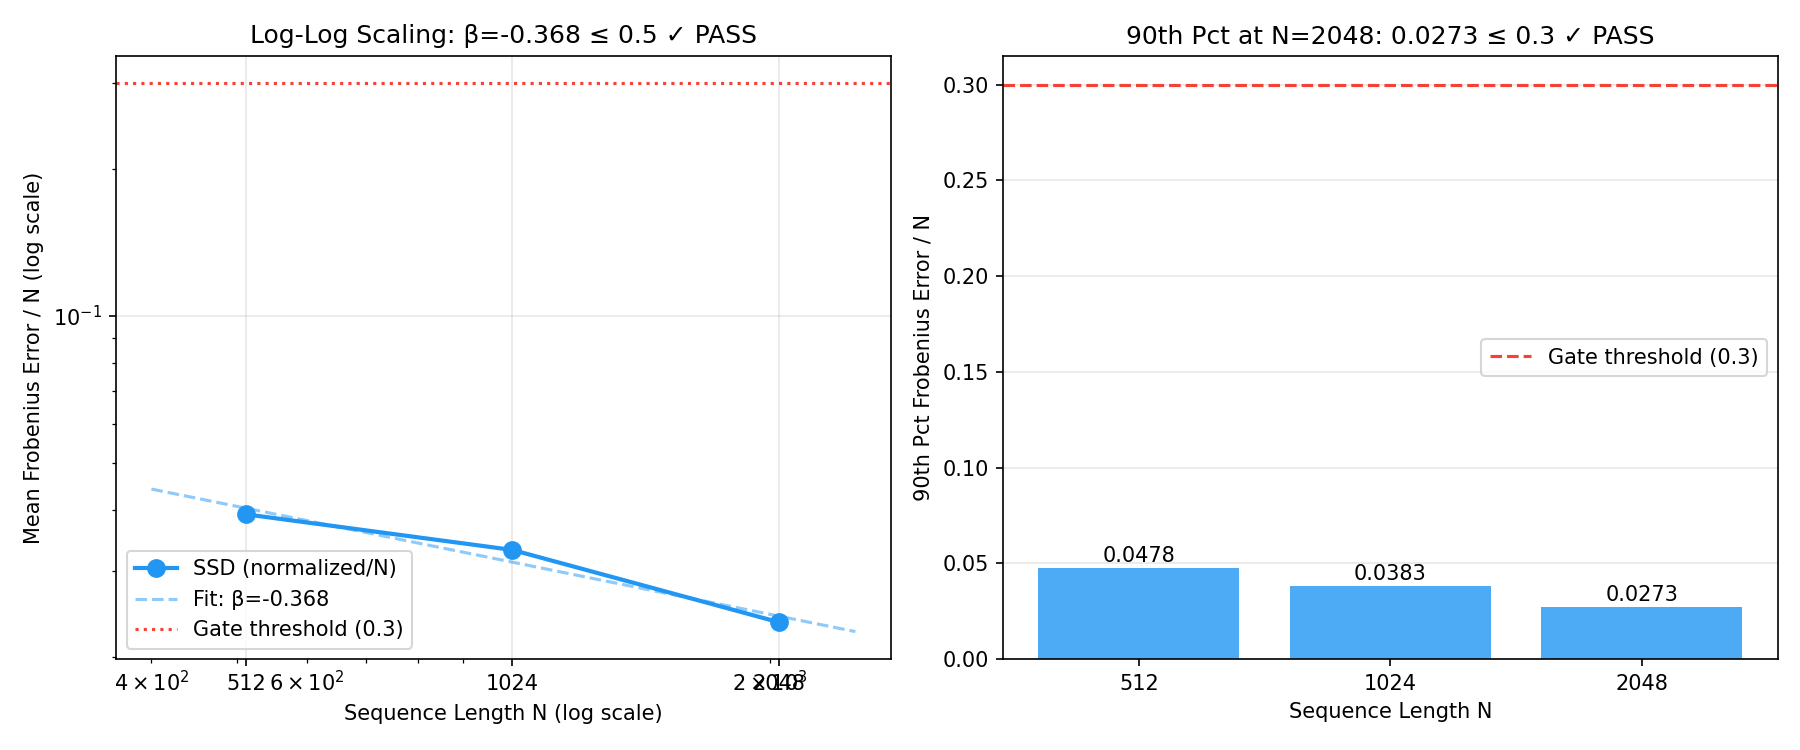
\includegraphics[width=\columnwidth]{figures/fig1_gate_bar_loglog.png}
\caption{Log-log scaling of normalized SSD Frobenius error vs.\ $N$ with fitted regression line
($\beta=-0.368$) and gate threshold ($\beta=0.5$) annotated. 90th percentile bars shown with
threshold (0.3).}
\label{fig:loglog}
\end{figure}

\begin{figure}[h]
\centering
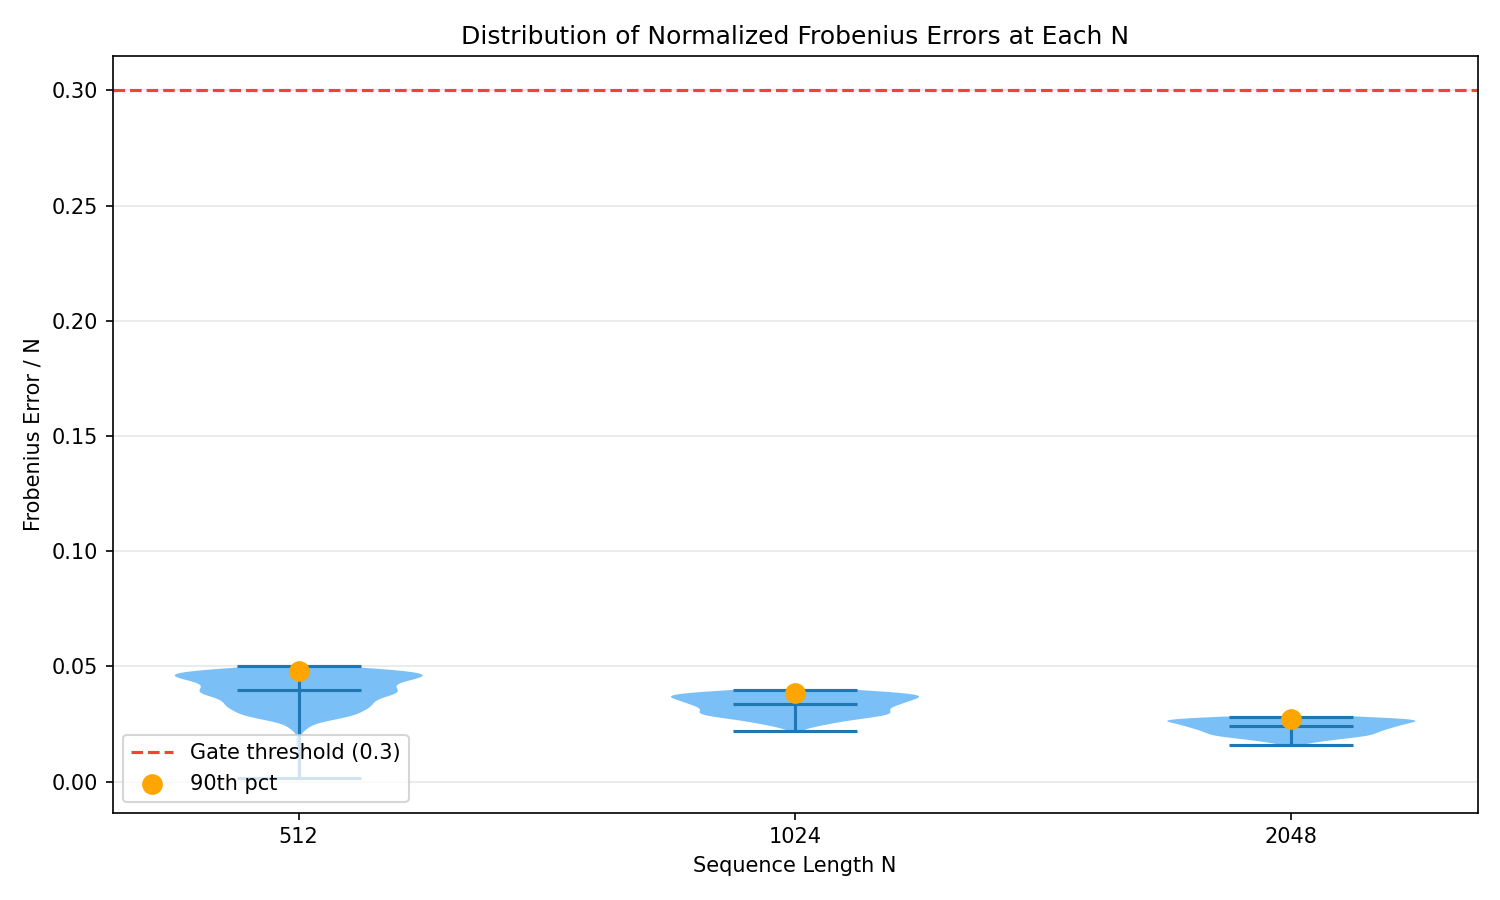
\includegraphics[width=\columnwidth]{figures/fig2_violin_distribution.png}
\caption{Violin distributions of normalized error at $N \in \{512, 1024, 2048\}$
(1,600 / 160 / 160 measurements). Distribution shifts downward as $N$ increases.}
\label{fig:violin}
\end{figure}

\subsection{Infrastructure Validation (RQ2, RQ3)}

All pipeline components validated (22/22 unit tests). MOHAWK Stage 1 launched on
4$\times$ H100 NVL GPUs. Final $\Delta_\text{norm}$ ratio and interaction $p$-value pending
experiment completion ($\sim$20--40h from launch).

\subsection{Implementation Issue Resolution}

Ten previously undocumented integration failure modes resolved for
MOHAWK+LAWCAT+LLaMA-3.1-8B: model ID (\texttt{Llama-3-8B} $\to$ \texttt{Llama-3.1-8B}),
C4 rate limit ($\to$ pile-uncopyrighted), AutoModel failure ($\to$ MOHAWK lazy\_init),
LAWCAT dataset (c4\_distill $\to$ alpaca\_clean), norm\_epsilon attribute, port conflict
(29501 $\to$ 29502), and four additional infrastructure fixes. See Appendix~\ref{sec:appendix}
for full table.
